\documentclass[11pt,letterpaper]{article}
\usepackage[top=0.85in,left=1.10in,footskip=0.75in]{geometry}
\usepackage[titletoc,page]{appendix}
% Use adjustwidth environment to exceed column width (see example table in text)
\usepackage{changepage}
\usepackage[english]{babel}
\usepackage{booktabs}
\usepackage{siunitx}%Questo serve a caricare il pacchetto delle unità di misura del sistema internazionale%
\usepackage[utf8]{inputenc}
\usepackage{graphicx} 
\usepackage{url}
\usepackage{amsmath}
\usepackage{amssymb}
\usepackage{listings}


\usepackage{keyval}
\usepackage{xcolor}
\usepackage{caption}
\usepackage{tikz}
\usepackage{circuitikz}
\usepackage{authblk}
%\usepackage{hyperref}


\usepackage[lofdepth,lotdepth]{subfig}
% Remove comment for double spacing
%\usepackage{setspace} 
%\doublespacing
% Text layout
%\raggedright
\setlength{\parindent}{0.5cm}
\textwidth 5.25in 
\textheight 8.75in

\usepackage[aboveskip=1pt,labelfont=bf,labelsep=period,justification=raggedright,singlelinecheck=off]{caption}

% Use the PLoS provided BiBTeX style
\bibliographystyle{plos2009}

% Remove brackets from numbering in List of References
\makeatletter
\renewcommand{\@biblabel}[1]{\quad#1.}
\makeatother


\begin{document}
\vspace*{0.30in}

\begin{flushleft}
{\Large
\textbf\newline{\textbf{Metropolis Monte Carlo and Crooks F. T.}}
}
\newline
% Insert Author names, affiliations and corresponding author email.
\\
Lorenzo Maria Perrone\textsuperscript{1, *}
%Name2 Surname\textsuperscript{2,\textpilcrow},
%Name3 Surname\textsuperscript{2,\textcurrency a},
%Name4 Surname\textsuperscript{2,\ddag},
%Name5 Surname\textsuperscript{2,\ddag},
%Name6 Surname\textsuperscript{2,\Yinyang},
%Name7 Surname\textsuperscript{3,*,\Yinyang}
\\
\bf{1} Department of Physics, EPFL
\\
%\bf{2} Affiliation Dept/Program/Center, Institution Name, City, State, Country
%\\
%\bf{3} Affiliation Dept/Program/Center, Institution Name, City, State, Country
%\\

% Insert additional author notes using the symbols described below. Insert symbol callouts after author names as necessary.
% 
% Remove or comment out the author notes below if they aren't used.
%
% Primary Equal Contribution Note
%\Yinyang These authors contributed equally to this work.

% Additional Equal Contribution Note
%\ddag These authors also contributed equally to this work.

% Current address notes
%\textcurrency a Insert current address of first author with an address update
% \textcurrency b Insert current address of second author with an address update
% \textcurrency c Insert current address of third author with an address update

% Deceased author note
%\dag Deceased

% Group/Consortium Author Note
%\textpilcrow Insert Collaborative Author line here

* E-mail: lorenzo.perrone@epfl.ch
\end{flushleft}


\section{Exercise: Investigation of Crooks Equality}

\subsection{Point 1}
The first question to this exercise involves the simulation of the probability distribution of the position of a particle who is trapped in a box with periodic boundary conditions and subjected to a triangular well potential. Every instant $t$ the particle can move left, right or stay in the same position with equal probability.\\
 To simulate so, we generate a random number from a flat distribution between 0 and 1: if it is smaller than 1/3, then the particle will move left, if it is bigger than 2/3 the particle will move right, otherwise it will stay in its previous position. Every time the particle tries to move to a configuration with higher energy, we use Metropolis acceptance method: it consists of throwing another random number $\xi$ and comparing it to the boltzmann factor of the energy levels $exp(-(E_2 - E_1))$. The move is allowed only if $\xi$ is smaller than the above exponential.\\

We attach below the code used to compute the probability distribution for the equilibrium state. The code itself is already the generalization for the case of a moving potential, but it reduces to the equilibrium code for the case speed = 0 (actually \textit{speed} is an inverse of a speed and can assume values such as 4,8,... it is in fact the number of time intervals needed before moving the potential. The case speed = 0 has been added for shortness).\\


The resulting plot is shown in Fig. (1).

\begin{figure}
\centering
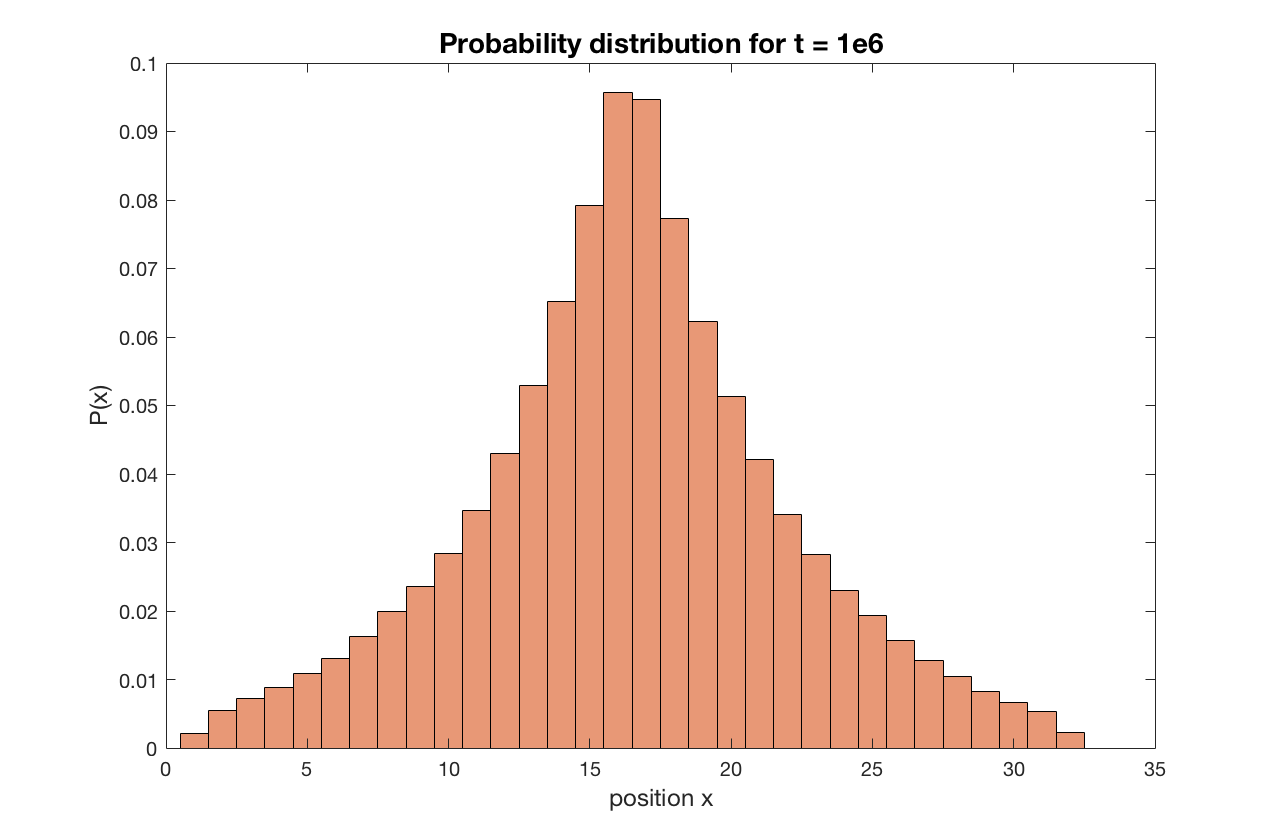
\includegraphics[width=0.9\linewidth]{./prob_equi}
\caption{Probability distribution for equilibrium problem}
\label{fig:prob_equi}
\end{figure}

\subsection{Point 2}
We now move to the case where the potential is shifted. However, although the code seems to be appropriately designed, results from different simulations vary a lot, not allowing us to confirm our implementation. Moreover, there could be a problem of velocity of convergence of the distribution to the PDF shown in Crooks [1999].\\
We report in Fig. (2 - 5) different simulations for a few speeds and times.

\begin{figure}
\centering
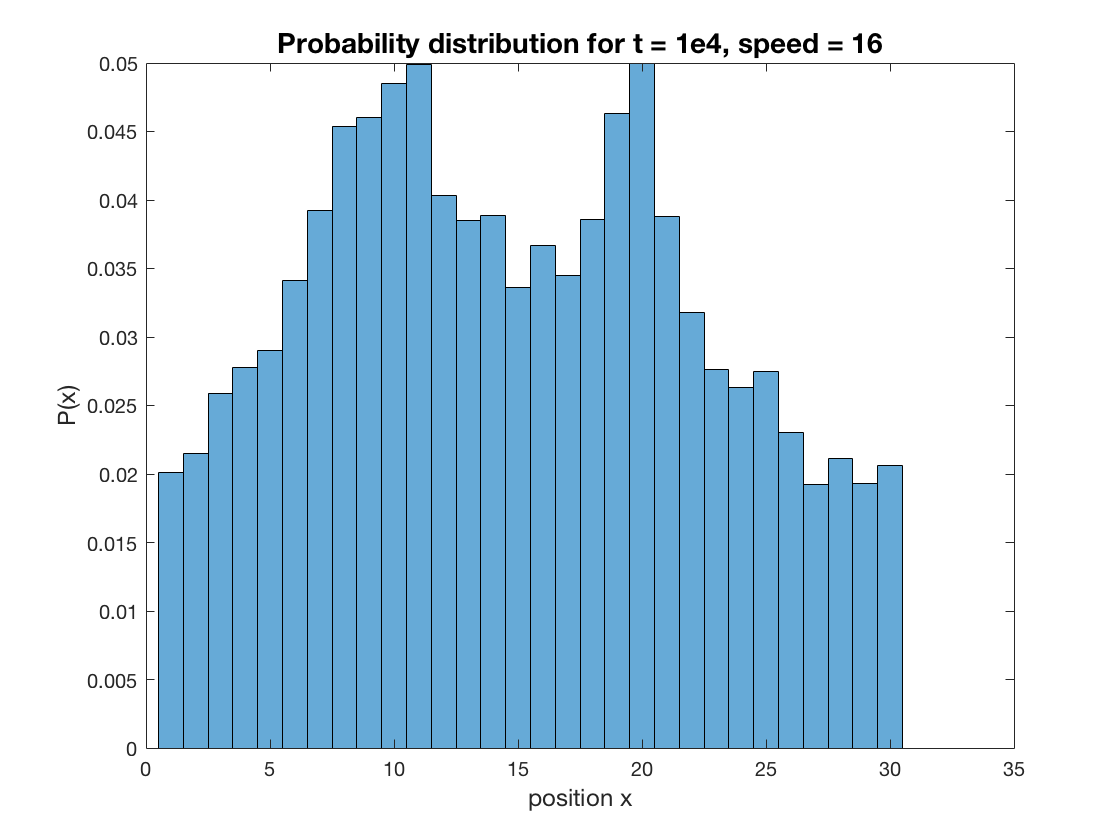
\includegraphics[width=0.9\linewidth]{./prob_6_1e4}
\caption{Probability distribution for speed = 16}
\label{fig:prob_16}
\end{figure}

\begin{figure}
\centering
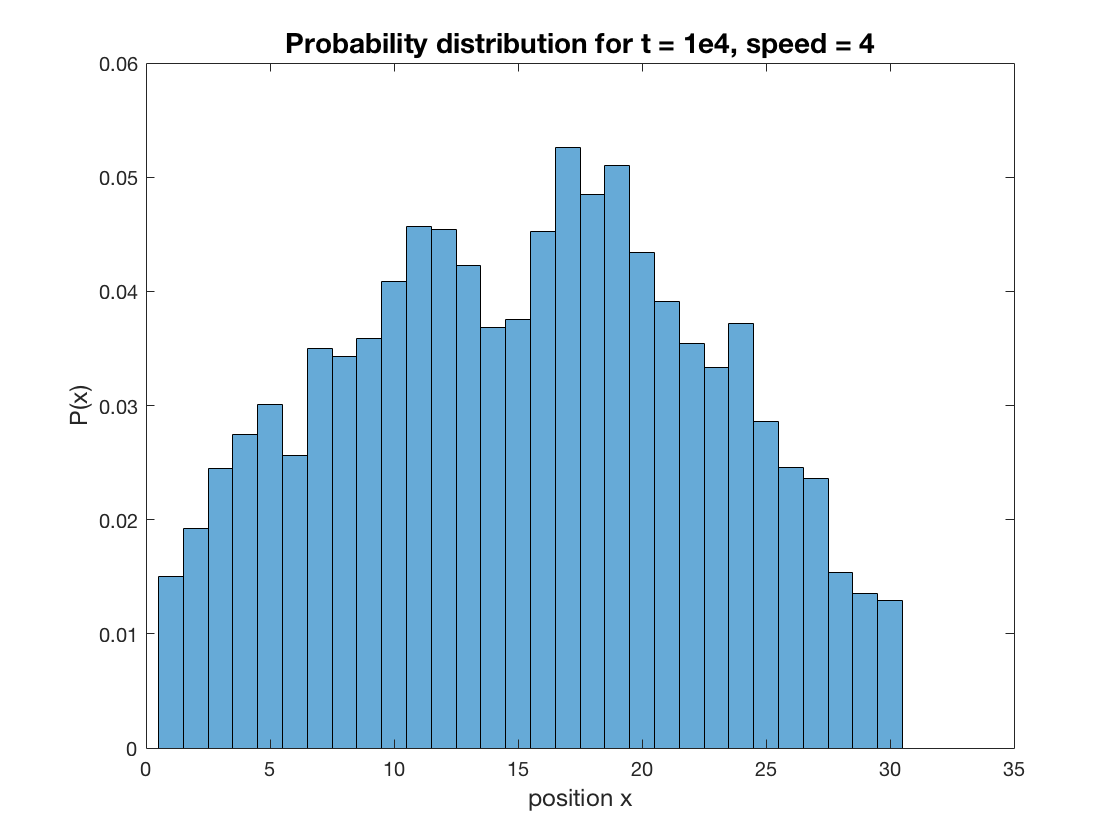
\includegraphics[width=0.9\linewidth]{./prob_4_1e4}
\caption{Probability distribution for speed = 4}
\label{fig:prob_4}
\end{figure}

\begin{figure}
\centering
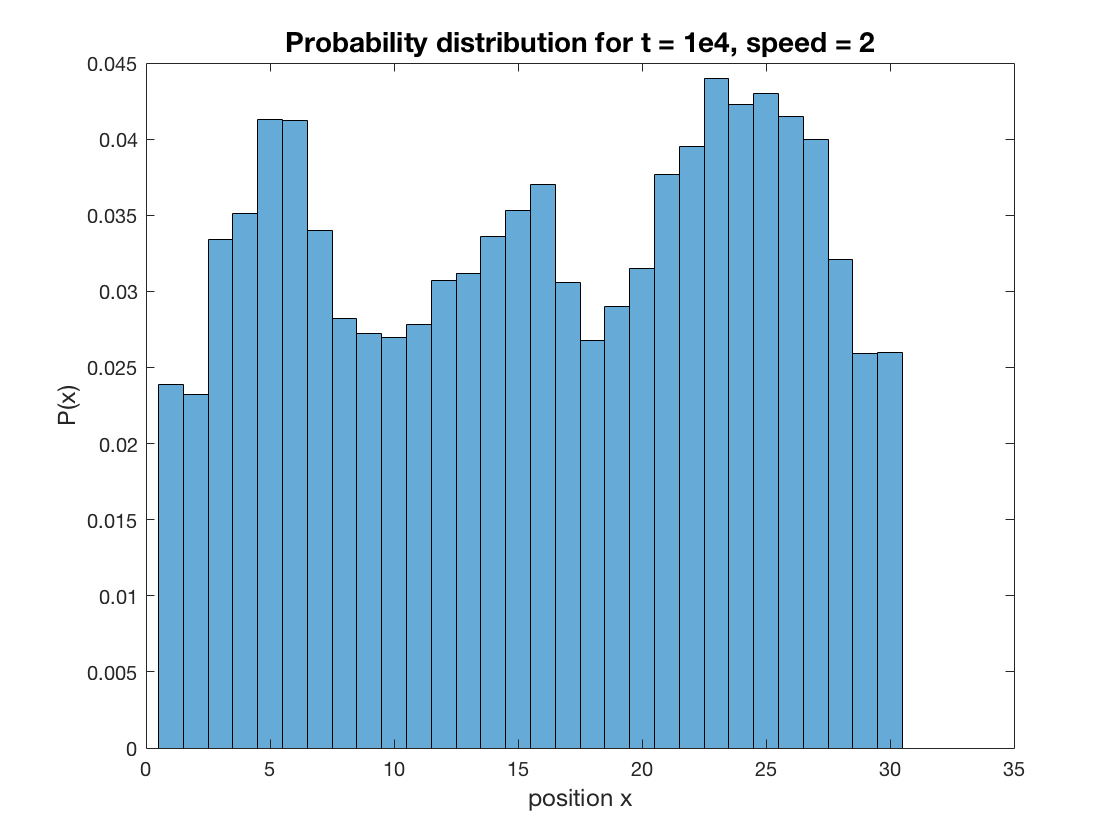
\includegraphics[width=0.9\linewidth]{./prob_2_1e4}
\caption{Probability distribution for speed = 2}
\label{fig:prob_2}
\end{figure}

\begin{figure}
\centering
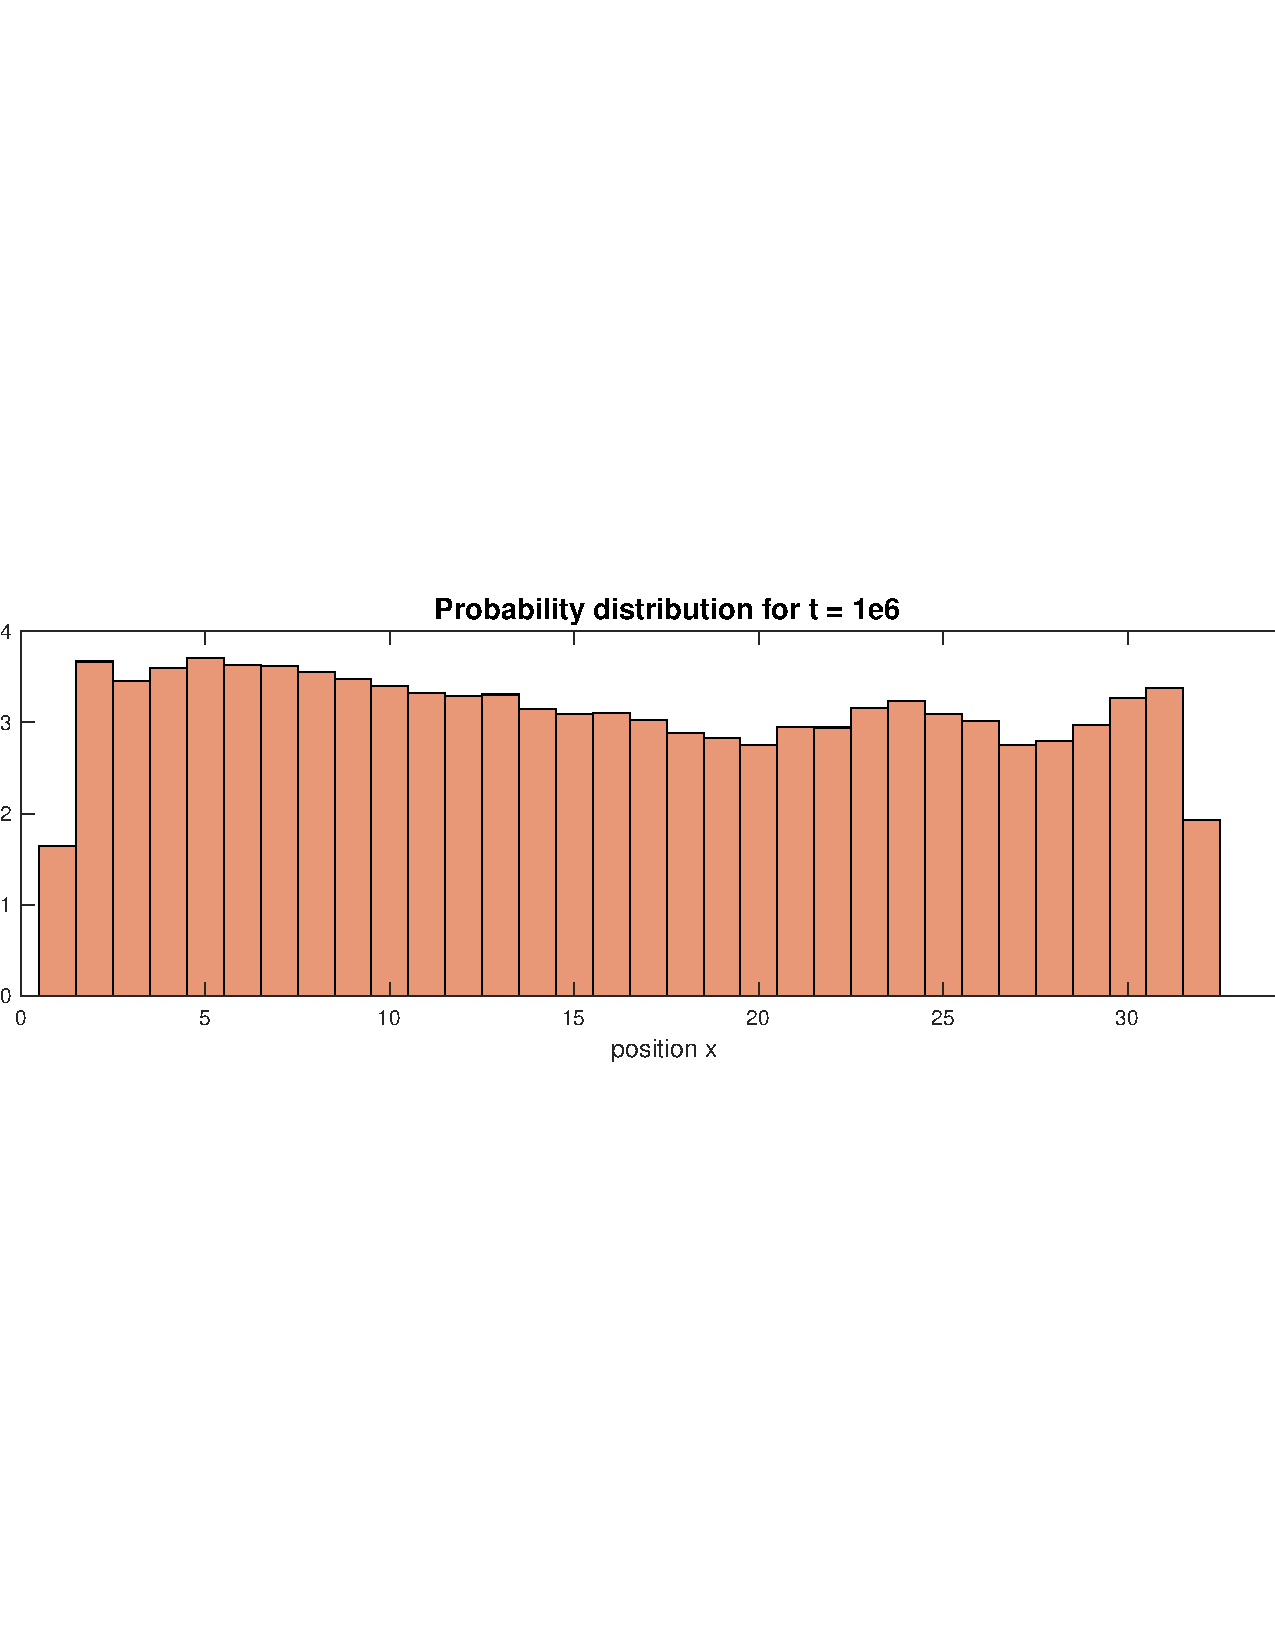
\includegraphics[width=0.9\linewidth]{./prob_1e6}
\caption{Probability distribution for speed = 8 and 1e6 time steps}
\label{fig:prob_8}
\end{figure}

It is not clear why the PDFs differ so sensibly from the one reported in Crooks paper. Moreover, it is not clear either how to extract values of W from this data: in fact, if we assume $W = E_f - E_i$ (because in a bath at thermal equilibrium there is no exchange of heat) we get inconsistent results as for the work probability distributions.

\begin{lstlisting}

@author: LorenzoLMP
"""
function [deltaH,x_position] = MMC(speed, deltat)
%speed is a parameter which tells after how many steps the potential is
%sshifted. However, for speed = 0 we obtain the equilibrium situation
time = deltat;
if speed ~=0
    N = ceil(time/(speed*31));
else
    N = 0;
end
%N is a number which is used in the definition of the triangular function.
%It tell how many triangles should be prepared so that the shifting works
%smoothly

%d defines the delay array for the triangular function, implemented as a
%tripulse
d = -(31*(N-1)+30):31:32;
kT = 5;
H = zeros(time,1); %energy of the configuration
x_position = zeros(time,1);
x_position(1) = randi(32,1,1);
H(1) = E(x_position(1),1);

for t = 2:time
    %the following piece is used to translate the coordinates every shift
    %of the potential, so as to be in the potential system of reference
    if (mod(t,speed)) == 0
            x_position(1:t-1) = x_position(1:t-1) - 1;
            x_position(x_position(1:t-1) < 1) = 30;
    end
    
    x_temp = 0;%displacement of the x coord
    r2 = rand(1,1);
        if r2<= 1/3
                 x_temp = -1;
        elseif r2 >= 2/3
                 x_temp = 1;
        end 
      %we hqve to take care of the boundary condition: 
      %if the particle
      %remains inside the box:
        if (x_temp ~=0) && (x_position(t-1) + x_temp <= 32) 
        && (x_position(t-1) + x_temp >= 1)
             %x_temp(x_temp>=1)= x_temp(x_temp>=1) -1;
            H_temp = E(x_position(t-1)+x_temp,t);  
            %we compare the energies of the configurations: all the
            %energies
            %are compared between t-1, x(t-1) and t, x(t)
            %now is the time to use metropolis acceptance
            if (H_temp > H(t-1))
                r = rand(1,1);
                     if r < exp(-(H_temp -H(t-1))/kT)
                              x_position(t) = x_position(t-1)+ x_temp;
                              H(t)=H_temp;
                     else
                              H(t) = E(x_position(t-1),t);
                              x_position(t) = x_position(t-1);
                     end
            % if energy decreases then particle moves automatically         
            elseif (H_temp <= H(t-1))
                x_position(t) = x_position(t-1)+ x_temp;
                H(t)=H_temp;
            end
        %if the particle moves outside, it re-enters 
        %from the other side    
        elseif (x_temp ~=0) && ((x_position(t-1) + x_temp > 32) 
        || (x_position(t-1) + x_temp < 1))
            %sort of same code here as before
            x1 = abs(x_position(t-1) + x_temp-31);
            H_temp = E(x1,t);    
            if (H_temp > H(t-1))
                r = rand(1,1);
                     if r < exp(-(H_temp -H(t-1))/kT)
                              x_position(t) = x1;
                              H(t)=H_temp;
                     else
                              H(t) = E(x_position(t-1),t);
                              x_position(t) = x_position(t-1);
                     end
                     
            elseif (H_temp <= H(t-1))
                x_position(t) = x1;
                H(t)=H_temp;
            end
            
        %if the particle does not move we simply update its energy 
        %(the potential might have moved) but same position    
        else
                H(t) = E(x_position(t-1),t); 
                x_position(t) = x_position(t-1);
        end 
        
        %this plots the shifted potential every speed steps. 
        %can be useful to debug
        if (mod(t,speed)) == 0
            figure;plot(linspace(1,32,1000),E(linspace(1,32,1000),t))
        end
        
end


%in the energy function the time parameter is passed so that the potential
%can be shifted every speed steps
function energy = E(x,t)
         s = 0;
         if speed ~=0
            s = floor(t/speed);
         end
         energy = 15*V(x,d+s,30);
end 

%this defines the triangular potential over the array defined at the
%beginning
function y = V(x,d,w)
    y = pulstran(x,d,'tripuls',w);
      
end


figure;histogram(x_position, 'Normalization', 'probability');
title('Probability distribution for t = 1e4, speed = 16', 'FontSize',14)
xlabel('position x', 'FontSize',12);ylabel('P(x)', 'FontSize',12);
end
\end{lstlisting}

\begin{lstlisting}
%This function is an attempt to retrieve the PDFs for 
%the work distributions starting from the energy differences
function work(deltat, iterations)
w_prob = zeros(iterations, 1);
    for i=1:iterations
        [deltaH,x_position] = MMC(8, deltat);
        w_prob(i) = deltaH;
    end
    figure;histogram(w_prob,'Normalization', 'probability');
end
\end{lstlisting}

\end{document}